\section{Problem Statement and System Model}
\label{sec:model}

\subsection{Problem Statement}
Consider a medical IoT deployment in which several institutions, such as
hospitals, surgical specialties or wearable installations, each hold
multimodal recordings of their own patients and wish to train a shared
prediction model. Every patient contributes many records, and no record may
leave its institution. The problem is to train the model through a
client--edge--cloud hierarchy such that
\begin{enumerate}
\item the participation of any single patient, with all of their records, is
protected by a formal $(\varepsilon,\delta)$ guarantee that covers every
message the system releases, edge tier included;
\item the model remains close in utility to an identical non-private system;
and
\item the system remains deployable on IoT infrastructure, with low uplink
traffic, reliable delivery, low inference latency and low energy.
\end{enumerate}
These requirements interact. Protecting patients instead of records reduces
the number of protected units and therefore raises the relative noise.
Clients partitioned by institution differ greatly in size, so a single noise
level fitted to the smallest client degrades every larger one. And an edge
tier changes how many optimization steps each client takes, and hence how
much of its budget it spends. The remainder of this section formalizes the
setting; Section~\ref{sec:method} addresses each difficulty in turn.

\subsection{System Model}
% Fig. 1 is defined here, one section early, so that it floats to the top of
% the page where Section IV cites it rather than a page later.
\begin{figure*}[!t]
\centering
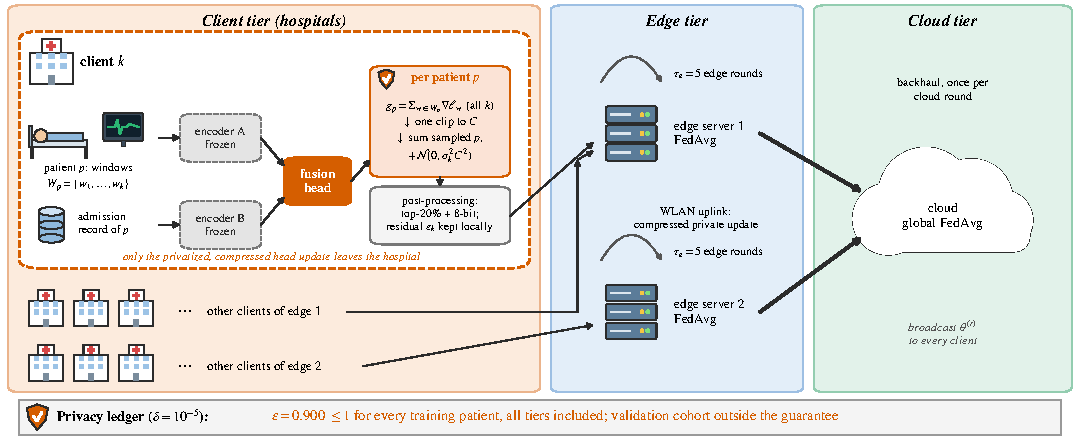
\includegraphics[width=\textwidth]{fig01_overview_core.pdf}
\caption{Architecture of PP-HFM. Clients train only the fusion head under patient-level DP; edges and the cloud average the noisy, compressed updates.}
\label{fig:overview}
\end{figure*}
A deployment has $K$ clients, such as hospitals, specialties or wearable
installations, assigned by a fixed public map $e(\cdot)$ to $E$ edge
aggregators, which report to one cloud aggregator (Fig.~\ref{fig:overview}). Client $k$ holds a dataset
$\mathcal{D}_k$ of $n_k$ records. Each record pairs two modalities of the same
individual over the same interval: modality~A is a multichannel time series
and modality~B a static or summarized feature vector. The records of client
$k$ are partitioned by individual into the patient set $\mathcal{P}_k$; patient
$p$ contributes the records $W_p$, with $k_p = |W_p|$. A patient's records
never span two clients or two evaluation splits; this holds by construction
for the eICU privacy-cost and end-to-end configurations, run on a
one-hospital-per-person partition, and for the person-level VitalDB partition
(Section~\ref{sec:setup}); the remaining eICU analyses use the source partition
and are qualified in Section~\ref{sec:method:analysis}. The model
$f_\theta$, with $\theta = (\theta_{\mathrm{enc}}, \theta_{\mathrm{head}})$,
comprises two modality encoders and a fusion head, and the learning objective
is the weighted empirical risk
\begin{equation}
\min_{\theta}\; F(\theta) = \sum_{k=1}^{K} \frac{n_k}{n}\,
\frac{1}{n_k}\!\!\sum_{(x,y)\in\mathcal{D}_k}\!\! \ell\big(f_\theta(x), y\big),
\label{eq:objective}
\end{equation}
with $n = \sum_k n_k$ and $\ell$ the unweighted cross-entropy; class weights
computed from training labels would be a further unprotected release.
Training runs for $R$ cloud rounds of $\tau_e$ edge rounds each.

Table~\ref{tab:notation} summarizes the notation.

\begin{table}[!t]
\centering
\caption{Notation}
\label{tab:notation}
\small
\begin{tabular}{ll}
\toprule
Symbol & Meaning \\
\midrule
$K$, $E$               & number of clients, of edge aggregators \\
$\mathcal{P}_k$, $W_p$ & patients of client $k$; records of patient $p$ \\
$k_p = |W_p|$          & records contributed by patient $p$ \\
$R$, $\tau_e$          & cloud rounds; edge rounds per cloud round \\
$B$, $q_k$             & expected patients per step; sampling rate \\
$C$, $\sigma_k$        & clipping norm; noise multiplier of client $k$ \\
$T_k$                  & optimization steps of client $k$ \\
$(\varepsilon,\delta)$ & privacy budget \\
\bottomrule
\end{tabular}
\end{table}

\subsection{Threat Model and Privacy Goal}
The adversary observes everything that leaves a client: every encoded update,
and every edge and cloud model. It may also
know all records except those of a target individual. Edge and cloud
aggregators are honest-but-curious and are treated as part of the adversary.
The goal is $(\varepsilon,\delta)$-differential privacy \cite{ref8} under the
\emph{patient-level} neighbouring relation: two datasets are neighbours if one
is obtained from the other by adding or removing \emph{all} records of a
single patient. A record-level guarantee, which removes one record, does not
meet this goal when $k_p > 1$. Public quantities are the architecture, the
pretrained encoder parameters, all hyperparameters, the edge map, the declared client
sizes $|\mathcal{P}_k|$ and $n_k$, and the input standardization constants,
which are fixed before training and are public only when fitted on the
disjoint pool (Table~\ref{tab:ledger}). The validation cohort, used to select the
reported checkpoint, is outside the guarantee, as is conventional
\cite{ref6}; Section~\ref{sec:method:analysis} lists every release.

\subsection{Research Objectives}
To make the three requirements testable, seven quantitative targets were fixed
before any experiment was run:
\begin{IEEEdescription}[\IEEEsetlabelwidth{O2b:}]
\item[O1:] reduce uplink traffic by at least $50\,\%$ relative to centralized
training;
\item[O1b:] reduce the latency of a training round relative to centralized
training;
\item[O2a:] keep the privacy budget at $\varepsilon \le 1$ for every protected
individual;
\item[O2b:] lose at most two points of utility relative to an identical
non-private system (cost = non-private minus private; a negative cost means
the private system scores higher);
\item[O3a:] keep the $95$th-percentile inference latency below $100$~ms;
\item[O3b:] deliver more than $99\,\%$ of updates; and
\item[O4:] save at least $20\,\%$ of energy per training round.
\end{IEEEdescription}
Section~\ref{sec:results:objectives} reports each target on every corpus.
